\begin{figure*}[t!]
\begin{center}
% \fbox{\rule{0pt}{2in} \rule{.9\linewidth}{0pt}}
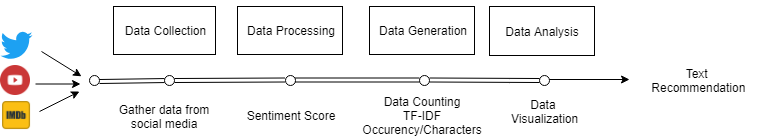
\includegraphics[width=0.8\linewidth]{img/Lexicon.png}
\end{center}
   \caption{Proposed approach overview: from data gathering to text recommendation.}
\label{fig:approach}
\end{figure*} 

The public opinion is one of the key factors for the success of a movie. To analyze and identify public opinion, we developed a sentiment analysis tool that, using tweets and comments from YouTube trailers, provides the following: \textit{i} The general public opinion about a movie; \textit{ii} The identification of the main topics on the evaluated texts; and \textit{iii} A ''recommendation text'' for the movie, based on the most relevant mentioned words. Next subsections describe all phases of the development to reach the proposed goal.

\subsection{Methodology}
\label{sec:Methodology}

Figure~\ref{fig:approach} presents our research methodology which is divided into five steps. The first one consists of collecting data from social media. On this step, we gathered data from both YouTube and Twitter, using the tools described in Subsection~\ref{sec:DataCollection}. Along with the scripts, this section details the data collection process as a whole.

After the Data Collection step, we executed the Data Processing step. During this second step, we used Vader to perform Sentiment Analysis on our texts.  This analysis provides us the sentiment scores and compound values for the tweets and comments collected. This step is fully detailed on Section \ref{sec:DataProcessing}
% I: não daria para complementar acima? Se eu entendi corretamentamente, no final do parágrafo acima poderia ter algo: Thus, we generate five files with the following content: (1) very positive; (2) positive; (3) neutral; (4) negative; and (5) very negative tweets and YouTube comments.
% Seria isto?



The fourth step of our study is the Data Analysis. On this step, we used the data generated data on the previous step to generate visualization charts. The goal of the visualization charts is to provide us information and statistics like the most frequent terms, the total of interaction, and others. Three visualization charts were generated on this step: a bar chart with the overall number of comments obtained, a word clouds presenting the most frequent words, and a heatmap showing the top 10 most used adjectives in movies comments. All these .visualizations are detailed described in Section \ref{sec:DataAnalysis}.


\subsection{Data Collection}
\label{sec:DataCollection}

For the context of movie reviews, we decided to analyze data from Twitter and YouTube comments about trailers. Twitter is used to quickly express opinions, and YouTube is a social media widely adopted to display movie trailers. We developed and used Python scripts to gather the desired data from the officials APIs of these social media. 

Twitter usually contain hashtags to indicate the subject of a text. Due to this reason, we chose to collect data through the use of hashtags instead of using keywords. We believe that the use of hashtags would provide a higher number of information and better quality data. The Twitter API implements features that allow a  user to provide a hashtag list with the subjects to be collected. Thus for each movie, we selected a different set of hashtags to be collected. 

The YouTube comments were collected from the Studios' officials channels. We collected data from all the officials' trailers released for a movie. In this analysis, we did not collect data from teasers. We only collect data from the top level of comments on YouTube. This decision was made because on the lower levels, the comments, generally, serve as an answer to previous comments and are not properly related to the movie. 

% I: estou em dúvida se o parágrafo abaixo não deveria ser o segundo parágrafo desta subseção. A ideia seria primeiro dizer como funcionam os scripts e depois explicar como foram feitas as coletas no contexto deste trabalho. Por exemplo, no Twitter foram usadas hashtags, e para o YouTube foram escolhidos os trailers oficiais dos studios. Trouxe para cá um texto que estava mais abaixo, e deixei os próximos dois parágrafos só com a descrição do que é coletado de cada rede social. Vejam se concordam com as alterações.
Both of our scripts are straight forward to use. The Twitter script just requires a list of hashtags to be collected and the YouTube script only requires the video ID. The video ID is easily spotted on its web address. The data collected from both scripts are stored on JSON files. The scripts used for data collection, along with a detailed description of how to use them, can be found on https://github.com/DAVINTLAB/TweetProcessing.

From Twitter, we collected data such as: \textit{username}, an internal user identification; \textit{lang}, the language in which the tweet was written; \textit{screen\_name}, user's name showed on screen; \textit{text}, the tweet written text; \textit{created\_at}, the date when the tweet was created; \textit{userid}, internal user identification; \textit{timezone}, the time zone in which the tweet was written; \textit{retweet\_count}, the number of times the tweet was re-posted; \textit{ID}, internal tweet identification; \textit{favorite\_count}, number of times other users liked this tweet.

From YouTube script, we collected the following data: \textit{publishedAt}, the date when the comment was posted; \textit{textOriginal}, the original comment text; \textit{likeCount}, the number of times another users liked the comment; and \textit{authorDisplayName}, the author name that is displayed on the screen. 

Besides the Twitter and YouTube scripts, we also developed a third script for the IMDB site. The main goal of this script is to provide a list of all the characters of a movie. Since the IMDB website does not provide an official API for this purpose, we used the free IMDBPY. API\footnote{https://imdbpy.sourceforge.io/}.

\subsection{Data Processing}
\label{sec:DataProcessing}

Sentiment analysis, also known as opinion mining, is a sub-field of Natural Language Processing (NLP)\cite{Indurkhya:2010}. The main purpose of Sentiment Analysis is to identify and extract impressions/opinions from a particular text~\cite{vader}. Although many improvements have already been done regarding the sentiment analysis area, this area still has opportunities for further enhancements, and so, there are several researches being developed for this area\cite{DEVIKA201644}.

Machine Learning is a widely used approach, and work by training an algorithm with a training data set, before applying it to the real data set\cite{DEVIKA201644}. This technique, first train the algorithm with some initials inputs, with known outputs, so that later it can work with new data\cite{He:2012}.

Lexicon based techniques work on the assumption that the collective polarity of a sentence or documents is the sum of polarities of individual phrases or words\cite{DEVIKA201644}. The term polarity lexicon is used to refer a dictionary or a vocabulary with the indications of positive and negative words with an associated score~\cite{Dipanjan:2016}. The difference between both approaches, is that the lexicon based does not need labeled data for testing\cite{DEVIKA201644}. 

% Classification techniques are based on word position, surrounding words, context analysis, part-of-speech, phrases, and others. 
Various lexicons may be used for this analysis. Examples are: AFINN Lexicon~\cite{afinn}\cite{anew}, Bing Liu's Lexicon~\cite{Jinda}, MPQA subjectivity Lexicon~\cite{Wilson}, SentiWordNet~\cite{esuli-sentiwordnet}\cite{baccianella-sentiwordnet}, Vader Lexicon~\cite{vader}, Pattern Lexicon~\cite{pattern}. 

In our research, we used Vader (Valence Aware Dictionary and sEntiment Reasoner)\footnote{https://github.com/cjhutto/vaderSentiment}
Lexicon to classify the tweets and comments from Youtube. In this approach, each word is labeled according to their semantic orientation as either positive or negative. Vader produces 4 sentiments metrics: the first three (positive, negative and neutral) represent the proportion of the words that match the categories. The final metric, \textit{compound} score, is a combination of the first three metrics normalized.
%SO normalizadas como?
The compound score ranges between -1 and 1, where -1 represents highly negative opinion and 1 highly positive opinion.

Since Vader deals with certain features that most of other lexicon do not (such as Abbreviations, Upper Case, Emojis, and Special characters), it is considered a very appropriate lexicon to be used in Social Media texts evaluation\cite{vader}. 
Through the example shown in Figure \ref{fig:tweet1}, we demonstrate the advantages of using Vader lexicon in Social Media.

%We consider using Vader Lexicon, to evaluate the tweets texts, for supporting the following aspects that non-normalized text may contain: Abbreviations, Upper Case, Emojis, Special characters. To understand, how Vader is great alternative to text analysis, follow a example: 

\begin{figure}[htb]
    \begin{center}
        
\includegraphics[width=0.8\linewidth]{img/Twitter1.png}
    \end{center}
       \caption{Example of a tweet post} %using Vader Lexicon.}
    \label{fig:tweet1}
\end{figure}

% I: acho que "tweet" já apareceu antes e não estava em itálico. Acho que não precisa colocar Tweet e Twitter em itálico. Revisar isso em todo o paper.
The tweet presented in Figure~\ref{fig:tweet1} was evaluated with the following scores for sentiment analysis: \textit{'compound'}: 0.6133, \textit{'neg'}: 0.169, \textit{'neu'}: 0.508, \textit{'pos'}: 0.322. As we can see, the overall evaluation of the text denotes a positive emotion. But if this same text was parsed without considering \textit{emojis} and the emotional indication represented by capital letters, 
%SO: mudei um pouco a frase acima para explicar o "capital letters".. mas na verdade não entendi esse parágrafo, fiquei com muitas duvidas. Joana, podes passar aqui?
the scores evaluation would be: \textit{'compound'}: 0.2043, \textit{'neg'}: 0.202, \textit{'neu'}: 0.546, \textit{'pos'}: 0.251. In this case, we can notice a significant drop on the \textit{compound} value, which makes the text's emotion tending to neutral, instead of positive.% as it should.
%SO: tens que explicar o que são esses parametros? compound indica o que?


\subsection{Dataset Generation}
\label{sec:DataGeneration}

\textit{Term Frequency-Inverse Document Frequency} indicates the weight of text's terms according to its frequency proportion~\cite{Dipanjan:2016} across documents. This is a well-known metric in information retrieval, and help us to identify the most recurrent terms in texts, allowing us to create visualization that work essentially with the use of words.

\begin{equation*}
    W_{t,d} = \left ( \frac{Freq_{t,d}}{Max} \right ) * log_2 \left ( \frac{N}{n_t} \right),
\end{equation*}
where \( W_{t,d}\) represents the term weight \textit{t} in document \textit{d}. 
\( Freq_{t,d}\) is the number of times that the terms ($t$) occurrences in document \textit{d}. 
\( Max\) is the total number of all words in document. 
\( N \) is how many times the term appears, \( n_t \) is number of documents containing the term \( t \). Applying the TF-IDF calculation, on the set of texts classified by Vader, we generate 5 outputs files, according to their polarity and with the structure as shown in the Listing \ref{tfidf}.

\begin{lstlisting}[label=tfidf,caption=TF-IDF File Structure,float,frame=tb]
    [('ragnarok', 'NN')],256
    [('saying', 'VBG')],2152
    [('rich', 'JJ')],125
    [('lots', 'NNS')],102
    [('much', 'JJ')],3509
\end{lstlisting}


%To understand how the public reacted to each character, it's necessary to have knowledge about the occurrences of the most used terms in relation to the main characters of a movie. This process is composed of 4 phases, as shown in Figure~\ref{fig:phases}. 
To understand how the public reacted to each character, it's necessary to know the number of occurrences of most used terms for each character. This process is consists of 4 phases, as shown in Figure~\ref{fig:phases}. 

For the first phase, we needed the list characters from the movie. So, we used the characters list generated by the IMDB script described in Section \ref{sec:DataCollection}. Then, for each character on
the list, we searched the set of texts classified by Vader % pelo q?
and store the texts that have this condition in a temporary list. On the third phase, we tried to find in the resulting TF-IDF files, the terms classified as adjectives which had at least 100 occurrences in texts. This result is also saved in a temporary list.  

%The last phase, is concerned with run the temporary list of text generated in phase 2, in the search for terms established in the phase 3. If condition is true, we add in a incremental variable, the number of times a given term is mentioned for each character, generating a occurrence file (Figure \ref{fig:occurs}). 
The last phase consists in %aqui
run the temporary list of text generated in phase 2, in the search for terms established in the phase 3. If condition is true, we add in a incremental variable, the number of times a given term is mentioned for each character, generating a occurrence file (Figure \ref{fig:occurs}). 

% 1 - lista de personagens
% 2 - textos classificados pelo vader, verifica se encontra os personagens da lista, se encontrar coloca em uma lista temporaria
% 3 - files tf-idf e busca so os adjetivos e guarda em lista temporaria 

\begin{figure}[h]
    \begin{center}
        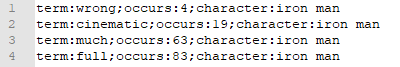
\includegraphics[width=0.8\linewidth]{img/occurs.png}
    \end{center}
       \caption{Occurrence File.} 
    \label{fig:occurs}
\end{figure}

\begin{figure*}[btp]
\begin{center}
% \fbox{\rule{0pt}{2in} \rule{.9\linewidth}{0pt}}
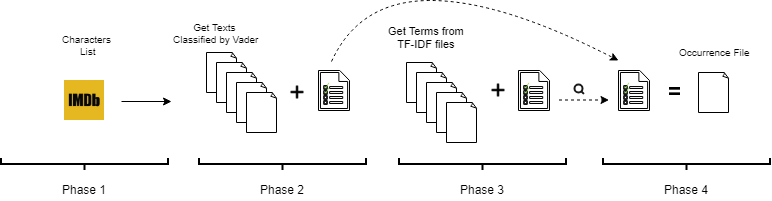
\includegraphics[width=0.8\linewidth]{img/diagrama-ocorrencia-movie.png}
\end{center}
   \caption{Occurrence Terms Model.}
\label{fig:phases}
\end{figure*}

\subsection{Data Analysis}
\label{sec:DataAnalysis}

For this paper, as mention before, we generated 3 visualization graphics for each social media we chose. The first one is a bar chart that displays the overall number of comments obtained for the selected movies on both social media. Each bar presented on this visualization represents one sentiment polarity (very positive, positive, negative and very negative). We opted to display the social media side by side to simplify users' comparison. 

The second visualization provides word clouds, showing the most used words for negative and positive sentiment polarity. For this visualization, we chose to use only verbs, noun, and adjective grammar types, because, for this case, we believe that those are the most significant ones. Like the previous visualization, 2 word clouds are generated for each social media, one for the most used words in negative comments, and another one for the most used words in positive comments. 

On the third visualization, a heatmap is presented. This visualization presents the top 10 most used adjectives in comments for the movie's characters. For this visualization, we present only characters for whom we were able to find mentions in the analyzed text. This visualization is split by sentiment polarity (positive and negative) and by social media (Twitter and YouTube). These visualizations can be seen in Figures ~\ref{fig:TotalOfInteractions},~\ref{fig:wordcloudsAquaman},~\ref{fig:wordcloudsCaptain},~\ref{fig:wordcloudsAvengers},~\ref{fig:AquamanCapitaHeatMap} and \ref{fig:VingadoresHeatMap}.

\subsection{Text Recomendation}
\label{sec:TextualRecomendation}


